% Options for packages loaded elsewhere
\PassOptionsToPackage{unicode}{hyperref}
\PassOptionsToPackage{hyphens}{url}
\PassOptionsToPackage{dvipsnames,svgnames,x11names}{xcolor}
%
\documentclass[
  letterpaper,
  DIV=11,
  numbers=noendperiod]{scrreprt}

\usepackage{amsmath,amssymb}
\usepackage{iftex}
\ifPDFTeX
  \usepackage[T1]{fontenc}
  \usepackage[utf8]{inputenc}
  \usepackage{textcomp} % provide euro and other symbols
\else % if luatex or xetex
  \usepackage{unicode-math}
  \defaultfontfeatures{Scale=MatchLowercase}
  \defaultfontfeatures[\rmfamily]{Ligatures=TeX,Scale=1}
\fi
\usepackage{lmodern}
\ifPDFTeX\else  
    % xetex/luatex font selection
\fi
% Use upquote if available, for straight quotes in verbatim environments
\IfFileExists{upquote.sty}{\usepackage{upquote}}{}
\IfFileExists{microtype.sty}{% use microtype if available
  \usepackage[]{microtype}
  \UseMicrotypeSet[protrusion]{basicmath} % disable protrusion for tt fonts
}{}
\makeatletter
\@ifundefined{KOMAClassName}{% if non-KOMA class
  \IfFileExists{parskip.sty}{%
    \usepackage{parskip}
  }{% else
    \setlength{\parindent}{0pt}
    \setlength{\parskip}{6pt plus 2pt minus 1pt}}
}{% if KOMA class
  \KOMAoptions{parskip=half}}
\makeatother
\usepackage{xcolor}
\setlength{\emergencystretch}{3em} % prevent overfull lines
\setcounter{secnumdepth}{5}
% Make \paragraph and \subparagraph free-standing
\makeatletter
\ifx\paragraph\undefined\else
  \let\oldparagraph\paragraph
  \renewcommand{\paragraph}{
    \@ifstar
      \xxxParagraphStar
      \xxxParagraphNoStar
  }
  \newcommand{\xxxParagraphStar}[1]{\oldparagraph*{#1}\mbox{}}
  \newcommand{\xxxParagraphNoStar}[1]{\oldparagraph{#1}\mbox{}}
\fi
\ifx\subparagraph\undefined\else
  \let\oldsubparagraph\subparagraph
  \renewcommand{\subparagraph}{
    \@ifstar
      \xxxSubParagraphStar
      \xxxSubParagraphNoStar
  }
  \newcommand{\xxxSubParagraphStar}[1]{\oldsubparagraph*{#1}\mbox{}}
  \newcommand{\xxxSubParagraphNoStar}[1]{\oldsubparagraph{#1}\mbox{}}
\fi
\makeatother


\providecommand{\tightlist}{%
  \setlength{\itemsep}{0pt}\setlength{\parskip}{0pt}}\usepackage{longtable,booktabs,array}
\usepackage{calc} % for calculating minipage widths
% Correct order of tables after \paragraph or \subparagraph
\usepackage{etoolbox}
\makeatletter
\patchcmd\longtable{\par}{\if@noskipsec\mbox{}\fi\par}{}{}
\makeatother
% Allow footnotes in longtable head/foot
\IfFileExists{footnotehyper.sty}{\usepackage{footnotehyper}}{\usepackage{footnote}}
\makesavenoteenv{longtable}
\usepackage{graphicx}
\makeatletter
\def\maxwidth{\ifdim\Gin@nat@width>\linewidth\linewidth\else\Gin@nat@width\fi}
\def\maxheight{\ifdim\Gin@nat@height>\textheight\textheight\else\Gin@nat@height\fi}
\makeatother
% Scale images if necessary, so that they will not overflow the page
% margins by default, and it is still possible to overwrite the defaults
% using explicit options in \includegraphics[width, height, ...]{}
\setkeys{Gin}{width=\maxwidth,height=\maxheight,keepaspectratio}
% Set default figure placement to htbp
\makeatletter
\def\fps@figure{htbp}
\makeatother
% definitions for citeproc citations
\NewDocumentCommand\citeproctext{}{}
\NewDocumentCommand\citeproc{mm}{%
  \begingroup\def\citeproctext{#2}\cite{#1}\endgroup}
\makeatletter
 % allow citations to break across lines
 \let\@cite@ofmt\@firstofone
 % avoid brackets around text for \cite:
 \def\@biblabel#1{}
 \def\@cite#1#2{{#1\if@tempswa , #2\fi}}
\makeatother
\newlength{\cslhangindent}
\setlength{\cslhangindent}{1.5em}
\newlength{\csllabelwidth}
\setlength{\csllabelwidth}{3em}
\newenvironment{CSLReferences}[2] % #1 hanging-indent, #2 entry-spacing
 {\begin{list}{}{%
  \setlength{\itemindent}{0pt}
  \setlength{\leftmargin}{0pt}
  \setlength{\parsep}{0pt}
  % turn on hanging indent if param 1 is 1
  \ifodd #1
   \setlength{\leftmargin}{\cslhangindent}
   \setlength{\itemindent}{-1\cslhangindent}
  \fi
  % set entry spacing
  \setlength{\itemsep}{#2\baselineskip}}}
 {\end{list}}
\usepackage{calc}
\newcommand{\CSLBlock}[1]{\hfill\break\parbox[t]{\linewidth}{\strut\ignorespaces#1\strut}}
\newcommand{\CSLLeftMargin}[1]{\parbox[t]{\csllabelwidth}{\strut#1\strut}}
\newcommand{\CSLRightInline}[1]{\parbox[t]{\linewidth - \csllabelwidth}{\strut#1\strut}}
\newcommand{\CSLIndent}[1]{\hspace{\cslhangindent}#1}

\KOMAoption{captions}{tableheading}
\makeatletter
\@ifpackageloaded{tcolorbox}{}{\usepackage[skins,breakable]{tcolorbox}}
\@ifpackageloaded{fontawesome5}{}{\usepackage{fontawesome5}}
\definecolor{quarto-callout-color}{HTML}{909090}
\definecolor{quarto-callout-note-color}{HTML}{0758E5}
\definecolor{quarto-callout-important-color}{HTML}{CC1914}
\definecolor{quarto-callout-warning-color}{HTML}{EB9113}
\definecolor{quarto-callout-tip-color}{HTML}{00A047}
\definecolor{quarto-callout-caution-color}{HTML}{FC5300}
\definecolor{quarto-callout-color-frame}{HTML}{acacac}
\definecolor{quarto-callout-note-color-frame}{HTML}{4582ec}
\definecolor{quarto-callout-important-color-frame}{HTML}{d9534f}
\definecolor{quarto-callout-warning-color-frame}{HTML}{f0ad4e}
\definecolor{quarto-callout-tip-color-frame}{HTML}{02b875}
\definecolor{quarto-callout-caution-color-frame}{HTML}{fd7e14}
\makeatother
\makeatletter
\@ifpackageloaded{bookmark}{}{\usepackage{bookmark}}
\makeatother
\makeatletter
\@ifpackageloaded{caption}{}{\usepackage{caption}}
\AtBeginDocument{%
\ifdefined\contentsname
  \renewcommand*\contentsname{Table of contents}
\else
  \newcommand\contentsname{Table of contents}
\fi
\ifdefined\listfigurename
  \renewcommand*\listfigurename{List of Figures}
\else
  \newcommand\listfigurename{List of Figures}
\fi
\ifdefined\listtablename
  \renewcommand*\listtablename{List of Tables}
\else
  \newcommand\listtablename{List of Tables}
\fi
\ifdefined\figurename
  \renewcommand*\figurename{Figure}
\else
  \newcommand\figurename{Figure}
\fi
\ifdefined\tablename
  \renewcommand*\tablename{Table}
\else
  \newcommand\tablename{Table}
\fi
}
\@ifpackageloaded{float}{}{\usepackage{float}}
\floatstyle{ruled}
\@ifundefined{c@chapter}{\newfloat{codelisting}{h}{lop}}{\newfloat{codelisting}{h}{lop}[chapter]}
\floatname{codelisting}{Listing}
\newcommand*\listoflistings{\listof{codelisting}{List of Listings}}
\makeatother
\makeatletter
\makeatother
\makeatletter
\@ifpackageloaded{caption}{}{\usepackage{caption}}
\@ifpackageloaded{subcaption}{}{\usepackage{subcaption}}
\makeatother

\ifLuaTeX
  \usepackage{selnolig}  % disable illegal ligatures
\fi
\usepackage{bookmark}

\IfFileExists{xurl.sty}{\usepackage{xurl}}{} % add URL line breaks if available
\urlstyle{same} % disable monospaced font for URLs
\hypersetup{
  pdftitle={Cálculo Numérico Modular},
  pdfauthor={Armando Handaya},
  colorlinks=true,
  linkcolor={blue},
  filecolor={Maroon},
  citecolor={Blue},
  urlcolor={Blue},
  pdfcreator={LaTeX via pandoc}}


\title{Cálculo Numérico Modular}
\author{Armando Handaya}
\date{2024-11-25}

\begin{document}
\maketitle

\renewcommand*\contentsname{Table of contents}
{
\hypersetup{linkcolor=}
\setcounter{tocdepth}{2}
\tableofcontents
}

\bookmarksetup{startatroot}

\chapter{Zeros de Funções}\label{zeros-de-funuxe7uxf5es}

Neste capítulo trataremos de métodos para resolver equações. E como toda
equação pode ser escrita por

\[f(x)=0\]

este assunto também é dito Zeros de Funções. Trataremos aqui de métodos
que resolve equações que satisfazem algumas poucas condições. Mas essa
restrição não invalida o esforço do estudo pois é grande a variedade de
equações que podem ser resolvidos pelos métodos apresentados. Começamos
definindo o zero de uma função.

\begin{tcolorbox}[enhanced jigsaw, toptitle=1mm, opacitybacktitle=0.6, arc=.35mm, breakable, left=2mm, leftrule=.75mm, title=\textcolor{quarto-callout-note-color}{\faInfo}\hspace{0.5em}{Zero/Raíz}, coltitle=black, colback=white, rightrule=.15mm, colframe=quarto-callout-note-color-frame, titlerule=0mm, bottomtitle=1mm, bottomrule=.15mm, toprule=.15mm, colbacktitle=quarto-callout-note-color!10!white, opacityback=0]

Seja \(f\) uma função e \(r\in Dom(f)\) um elemento no domínio de \(f\).
Este é dito um zero ou raíz da função se e somente se \[f(r)=0.\]

\end{tcolorbox}

Alguns exemplos de zeros de funções podemos ver na tabela abaixo.

\begin{longtable}[]{@{}cc@{}}
\toprule\noalign{}
função & zero \\
\midrule\noalign{}
\endhead
\bottomrule\noalign{}
\endlastfoot
\(f_1(x)=x^2-5x+3\) & 0,6972243623 \\
\(f_2(x)=-x^3-4x+3\) & 0,6735930582 \\
\(f_3(x)=\sqrt{x}-5e^{-x}\) & 1,43044508899 \\
\(f_4(x)=e^x+x\) & -0,56714329040 \\
\(f_5(x)=x lnx-1\) & 1,76322283304 \\
\end{longtable}

A função quadrática \(f_{1}(x)\) pode ser resolvida pela fórmula de
Bháskara \[x=\frac{-b\pm \sqrt{b^2-4ac}}{2a}\]

que fornece a resposta diretamente. A função cúbica \(f_{2}(x)\) pode
ser resolvida pela fórmula de Tartáglia, mas as demais funções dessa
lista não possuem fórmula alguma. Então como calcular os raízes delas ?
Até funções polinômiais de ordem maior que 4 não há fórmulas de
resolução. Dessa forma como se podemos resolver uma equação como
\[x^5+2x^2-x=0  ?\]

Neste capítulo, vamos aprender a resolver essa e outras equações que não
possuem fórmulas prontas de resolução.

Os métodos que aprenderemos aqui são chamados de Métodos Iterativos.
Isso por conta das iterações ou rodadas que fazemos para melhorar (ou
refinar) cada vez mais a raíz da equação. Raíz de uma equação é a
solução do problema em questão.

Diferentemente do Método Direto ou Analítico que usa uma fórmula como a
de Bháskara para resolver uma equação de 2º grau. Essa fórmula nos
fornece as raízes diretamente.

Métodos Iterativos são úteis para resolver equações que não possuem
fórmulas de resolução. E elas são, na verdade, a maioria. Para
determinar a raiz da equação pelo método iterativo existem algumas
etapas que devemos percorrer, a saber :

\begin{enumerate}
\def\labelenumi{\arabic{enumi}.}
\item
  Definir a precisão de conta.
\item
  Dar um chute inicial.
\item
  Escolher um Método de Refinamento.
\item
  Escolher um ou mais Critérios de Parada.
\item
  Executar o processo até satisfazer todos os critérios de Parada
  adotados.
\end{enumerate}

As quatro primeiras etapas normalmente são fornecidas no enunciado da
questão, embora isso não seja uma regra. Já a quinta etapa é a parte que
o aluno precisa fazer. É nesta etapa que o aluno será avaliado.

\section{Precisão}\label{precisuxe3o}

A precisão da conta é para definir a proximidade em relação à raiz.
Suponhamos que a raiz seja \(r=3,135104\). Consideremos os seguintes
números

\[\left\{\begin{matrix}
a_1 = 3,135199\\
a_2 = 3,135098
\end{matrix}\right.\]

cujas diferenças em módulo em relação a r são, respectivamente

\[\begin{array}{c}|a_{1}-r|=0,000095<10^{-4}\\|a_{2}-r|=0,000006<10^{-5}\end{array}.\]

Dizemos que a precisão de \(a_{1}\) é de \(\varepsilon=10^{-4}\) e a de
\(a_{2}\) é de \(\varepsilon=10^{-5}\), portanto \(a_{2}\) é mais
próxima à raiz e por isso é um resultado melhor. Entretanto, não
confunda a precisão com o número de casas decimais corretas. Observe que
\(a_{1}\) tem as primeiras 4 casas decimais corretas ao passo que
\(a_{2}\) apenas 3, embora seja um resultado melhor

\[\begin{array}{c}a_{1}=3,\underline{1351}99\\a_{2}=3,\underline{135}098\end{array}.\]

Outra maneira de se referir à precisão é dizer que \(a_{1}\) tem
precisão de 4 casas decimais e \(a_{2}\) tem a precisão de 5 casas
decimais. Isso tem a ver com o número de zeros na diferença para o valor
correto e não com o número de decimais corretas. Mas há casos em que o
enunciado pede justamente isso: decimais corretas até a \(n\)-ésima
casa. Por isso deve-se sempre prestar atenção no enunciado do problema!
Quando se pede isso, o exemplo acima nos dá uma ideia do que fazer :
aumentar a precisão em algumas casas decimais. Nesse exemplo vimos que
\(a_{2}\) tem a precisão de 5 casas, pois, \(\varepsilon=10^{-5}\), mas
acerta apenas as 3 primeiras casas decimais. Se o enunciado pedir 4
corretas, temos que trabalhar com uma precisão maior, talvez
\(\varepsilon=10^{-6}\). Mas, dependendo do dígito da \(n\)-ésima casa,
muitas vezes a precisão de \(n\) casas já é suficiente. Veja no exemplo
acima onde \(a_{1}\) tem precisão de 4 casas e acertando as 4 decimais
iniciais. Em geral, uma precisão de \(n+1\) casas já serve para acertar
as \(n\) decimais iniciais. Mas isso nem sempre acontece. Quando há a
presença de zeros no valor exato, por exemplo, pode dar problemas.
Vejamos um exemplo. Suponhamos que o valor correto seja \[r=3,121002.\]
Com a precisão de 5 casas e obtemos os seguintes resultados
\[\begin{array}{c}a_{1}=3,\underline{12}0993\\a_{2}=3,\underline{1210}10\\a_{3}=3,\underline{12100}9\end{array}\]
Verifique que todos têm a mesma precisão de \(\varepsilon=10^{-5}\) mas
os números \(a_{1},a_{2},a_{3}\) acertam, respectivamente, duas, quatro
e cinco casas decimais. Uma observação a fazer aqui é a seguinte: quando
se pede n decimais corretas, não significa qualquer decimais mas sempre
as primeiras decimais a partir da vírgula.

\section{Chute Inicial}\label{chute-inicial}

Caso o valor inicial não seja fornecido, você mesmo deve fazer esse
chute. Depois, é só rodar o programa e veja se ele converge para algum
ponto fixo. Esse ponto fixo será a raiz do problema. Um bom chute
inicial faz o processo convergir para algum lugar. Esse lugar que
falamos é um valor cujo processo modifica muito pouco os seus dígitos,
talvez só na décima primeira casa decimal. Por isso o chamamos de ponto
fixo.

Mas, como podemos saber se o chute inicial que fizemos foi bom ou não ?
Essa é uma boa pergunta. Normalmente se você começar por um ponto mais
ou menos próximo à raiz, será um bom chute. Mas pode acontecer que o
chute não seja tão perto da raiz, mesmo assim converge para um ponto
fixo. Então não se preocupe muito com isso. Basta você rodar o programa
e ver se converge. Se não convergir, tente outro chute e recomece o
processo.

\section{Método de Refinamento}\label{muxe9todo-de-refinamento}

A segunda etapa é escolher um método de refinamento. Esse método por
vezes também é uma exigência do professor/examinador. Mas quando não é
fornecido ou não é exigido, você pode escolher qualquer um dos métodos
ensinados e aprendidos.

\section{Critérios de Parada}\label{crituxe9rios-de-parada}

Neste texto vamos usar dois critérios de parada, um para cada variável.
Por que isso ? Lembramos que estamos trabalhando com duas variáveis,
\(x\) e \(y\), a segunda dependente da primeira, ou seja \(y=f(x)\).
Dizemos que \(y\) é a imagem de \(x\) e que \(x\) é abscissa de \(y\).
Também se diz de \(y\) como ordenada de \(x\) e \(x\) como pré-imagem de
\(y\). Lembrando que, uma raiz de \(f\) é um valor \(x=r\) tal que
\(y=f(r)=0\). Assim queremos achar um valor da variável \(x\)
determinado pelo valor 0 da outra variável: \(y\). Quem pode-me garantir
que um valor próximo à raiz tem imagem próxima de zero ? Veja por
exemplo a função

\[f(x)=5000x^2-300\]

cuja raíz positiva é \(r=0,24495\). O valor \(a=0,244\) é bastante
próxima à raiz com precisão de \(0,00095<\varepsilon=10^{-3}\) mas a
imagem dele é longe de zero, pois \(f(a)=-2,32\) . Na verdade, qualquer
função cujo gráfico é quase vertical na raiz vai dar esse problema.

\begin{figure}[H]

{\centering 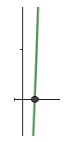
\includegraphics{Casivertical.png}

}

\caption{Gráfico da função \(f(x)\)}

\end{figure}%

Dessa forma, vamos adotar dois critérios de parada. Para a variável x
devemos garantir que

\[|x-r|<\varepsilon\]

e para a variável \(y=f(x)\) vamos adotar o critério

\[|f(x)|<\varepsilon\] e usaremos a mesma precisão para ambos os
critérios. Mas observe que há um grande problema no primeiro critério de
parada, pois não sabemos o valor exato de \(r\). Justamente esse valor
de \(r\) que estamos procurando. Portanto precisamos trocá-lo por outro
critério tangível. Há duas formas de fazer isso. O primeiro deles é
calcular a melhora dos passos da sequência de iterações (também chamado
de erro absoluto). \[|x_{i}-x_{i+1}|<\varepsilon\]

A segunda maneira é calcular a ``porcentagem'' de melhora desses passos
ou mais precisamente a taxa de melhora dos passos (também chamado de
erro relativo), dada por

\[\left|\frac{x_{i}-x_{i+1}}{x_{i+1}}\right|<\varepsilon\]

Essa segunda fórmula é mais sensível a erros, pois em nenhum momento a
sequência de iterações pode atingir o valor zero. Pois senão estaríamos
dividindo por zero. Aliás, essa também é a razão porque se coloca
\(x_{i+1}\) no denominador, e não \(x_{i}\), pois na maioria das vezes o
valor inicial que adotamos é o zero. Se assim for, o processo já começa
com problema.

Diante do exposto vamos adotar o critério de melhora dos passos para
garantir a aproximação da abscissa x à raiz em questão.

Um terceiro critério de parada seria o número máximo de iterações.
Existem casos em que o processo de refinamento não converge para nenhum
lugar. Nesses casos nenhum dos critérios anteriores serão satisfeitos,
mas o processo precisa parar de alguma forma. Para isso pode-se adotar o
número máxima de iterações como outro critério de parada. Isso é
necessário quando o processo é implementado em um sistema automático,
como em computador. Quando o processo é executado manualmente o número
máximo de iterações não deve ser muito alto, talvez no máximo uma dúzia
de iterações ou próximo disso. Hoje em dia com o recurso do computador
esse número máximo pode ser um milhão ou mais. Mas neste caso o problema
passa a ser o esforço humano. Acredito que ninguém vai fazer um milhão
de rodadas a não ser que saiba automatizar esse processo. Para isso você
deve saber e usar uma linguagem de programação, o que complica mais o
aprendizado. Mesmo assim, acredito que se um processo atingir um milhão
de rodadas \ldots{} muito provavelmente ele não vai convergir a lugar
nenhum. Então porque raios devemos executar tantas rodadas ? Como disse
antes, se você rodar e depois de umas cinquenta rodadas, ou até menos,
ele não atinge um ponto fixo .. você deve começar a desconfiar que o
processo não converge. Neste caso, descarte tudo e comece novamente com
outro chute inicial. Simples assim. Por este motivo também que não vamos
adotar esse terceiro critério de parada.

\section{Execução do Processo}\label{execuuxe7uxe3o-do-processo}

A fase de execução do processo é aquela que o aluno precisa mostrar na
prova/exame. Neste texto a execução do processo não será feita
manualmente e nem tampouco automaticamente. Vamos implementar sim em um
computador mas o processo não será executado automaticamente, mas sim
iteração por iteração. Por isso mesmo não vamos precisar impor o número
máximo de iterações como um critério de parada. Vamos avaliar a
continuidade do processo ou não a cada nova iteração.

A execução do processo será feita no computador usando softwares
específicos. No caso de zeros de funções, assunto deste capítulo, vamos
usar uma planilha eletrônica tais como Excel, Calc, Google Planilhas ou
Geogebra. Cada iteração corresponde a uma linha da planilha.

No capítulo 2, quando falamos de ajuste de curvas, vamos usar o Matlab,
Scilab, Octave ou Geogebra. Mas nesse capítulo o processo não será
iterativo, senão analítico. Uma única iteração basta para resolver o
problema.

No capítulo 3, falamos de Interpolação Polinomial. Nele vamos usar o
software Geogebra e o processo também não será iterativo.

No capítulo 4. abordaremos a Integração Numérica, e voltaremos a usar
uma planilha eletrônica. Mas o processo também não será iterativo.

No capítulo 5 passaremos a abordar Sistemas Lineares e vamos voltar a
usar uma planilha eletrônica. Nesse capítulo o processo será iterativo.

Então vamos começar com o primeiro método iterativo numérico.

\section{Método da Bissecção}\label{muxe9todo-da-bissecuxe7uxe3o}

Este método consiste em refinar intervalos que chamamos aqui de
intervalos de bolzano. Cada iteração corta o intervalo pela metade, mas
de forma que a propriedade da presença da raiz seja preservada. Nessa
sequência de cortes, uma hora o tamanho do intervalo e consequentemente
os candidatos à raiz será menor do que um valor ɛ previamente definido.
Vamos começar apresentando o Teorema de Bolzano.

\begin{tcolorbox}[enhanced jigsaw, toptitle=1mm, opacitybacktitle=0.6, arc=.35mm, breakable, left=2mm, leftrule=.75mm, title=\textcolor{quarto-callout-note-color}{\faInfo}\hspace{0.5em}{Teorema de Bolzano}, coltitle=black, colback=white, rightrule=.15mm, colframe=quarto-callout-note-color-frame, titlerule=0mm, bottomtitle=1mm, bottomrule=.15mm, toprule=.15mm, colbacktitle=quarto-callout-note-color!10!white, opacityback=0]

Seja \(f\) uma função contínua num intervalo fechado \([a,b]\) talque
\(f(a)f(b)<0\). Então \(f\) possui uma raiz no intervalo \([a,b]\).

\end{tcolorbox}

O intervalo fechado significa que ele é delimitado pelas suas
extremidades : \(a\) e \(b\). Consequentemente, o gráfico da função
também tem extremidades. O teorema garante que se a função é contínua e
as extremidades do gráfico estão em lados opostos do eixo x, então o
gráfico cruza o eixo x em algum ponto do intervalo.

Sejam dados um intervalo inicial de Bolzano \(I_{0}=[a_{0},b_{0}]\) e
uma precisão ɛ. O primeiro candidato à raiz é o seu ponto médio

\[x_{0}=\frac{a_{0}+b_{0}}{2}\] que divide o intervalo \(I_{0}\) em duas
metades. Se o ponto médio não for a raíz então ela deve estar em uma das
metades, conforme diz o Teorema. A metade que mantêm a propriedade de
Bolzano, ou seja as extremidades do gráfico em lados opostos, será o
novo intervalo de Bolzano \(I_{1}\), cujo tamanho é a metade do
anterior.

Repete-se esse procedimento até satisfazer os critérios de parada ou o
ponto médio acertar a raíz. Os critérios de parada que usaremos são

\[|f(x_{i})|<\varepsilon\] e \[|x_{i+1}-x_{i}|<\varepsilon.\]

O segundo critério, passo menor que \(\varepsilon\), pode ser trocado
por: intervalo \(\left|I_{i+1}\right|<\varepsilon\). Lembrando que
\(x_{i}\) é uma das extremidades do intervalo \(I_{i+1}\) e \(x_{i+1}\)
é o seu ponto médio. Por isso o tamanho do intervalo \(I_{i+1}\) é
exatamente o dobro do passo \(|x_{i+1}-x_{i}|\).

Na Figura Figure~\ref{fig-SeqInt} vemos uma ilustração do Método da
Bissecção, que consiste em uma sequência de Intervalos de Bolzano cada
vez menores mas sempre contendo a raiz da função f.~O intervalo seguinte
será sempre a metade do atual e o ponto de corte é o seu ponto médio. A
estimativa para a raíz em cada intervalo é esse ponto médio.

Esse método da Bissecção em formato de algoritmo pode ser visto abaixo.
A sua implementação pode ser feita em uma planilha eletrônica. Visando
favorecer a legibilidade de informações, porém, adotamos uma precisão
específica, tomada aleatoriamente, de 3 casas decimais e escolher o
subintervalo à esquerda do ponto médio para testar a condição de
Bolzano. Uma alternativa para fazer o teste de Bolzano seria o
subintervalo à direita do ponto médio.

\begin{center}\rule{0.5\linewidth}{0.5pt}\end{center}

\begin{tcolorbox}[enhanced jigsaw, toptitle=1mm, opacitybacktitle=0.6, arc=.35mm, breakable, left=2mm, leftrule=.75mm, title={Algoritmo da Bissecção}, coltitle=black, colback=white, rightrule=.15mm, colframe=quarto-callout-important-color-frame, titlerule=0mm, bottomtitle=1mm, bottomrule=.15mm, toprule=.15mm, colbacktitle=quarto-callout-important-color!10!white, opacityback=0]

Dada uma função \(f(x)\) contínua, um valor minúsculo \(\varepsilon\) e
um intervalo de Bolzano inicial \((a_{0},b_{0})\), para localizar uma
raíz nesse intervalo cortamos seguidamente esse intervalo pela metade da
seguinte maneira

\begin{enumerate}
\def\labelenumi{\arabic{enumi}.}
\item
  O intervalo atual sendo \((a_{i},b_{i})\) chamamos de Ponta-Esquerda
  (PE) e Ponta-Direita (PD) as extremidades \(a_{i}\) e \(b_{i}\),
  respectivamente. Seja \(x_{i}\) o ponto médio do intervalo. Se o
  tamanho do intervalo e a distância de \(f(x_{i})\) ao zero forem
  menores do que \(\varepsilon\), isto é
  \(\|\mbox{PD-PE}\|<\varepsilon\) e \(\|f(x_{i})\|<\varepsilon\), então
  pare aqui e a raíz aproximada será \(x_{i}\).
\item
  Se \(f(x_{i})=0\) então pare aqui e a raíz exata será \(x_{i}\). Caso
  contrário tome como o novo intervalo \((a_{i+1},b_{i+1})\) uma das
  metades do intervalo, ou seja \([PE,x_{i}]\) ou \([x_{i} ,PD]\),
  aquele que seja um intervalo de Bolzano. Volte ao passo 1.
\end{enumerate}

\end{tcolorbox}

\begin{figure}

\centering{

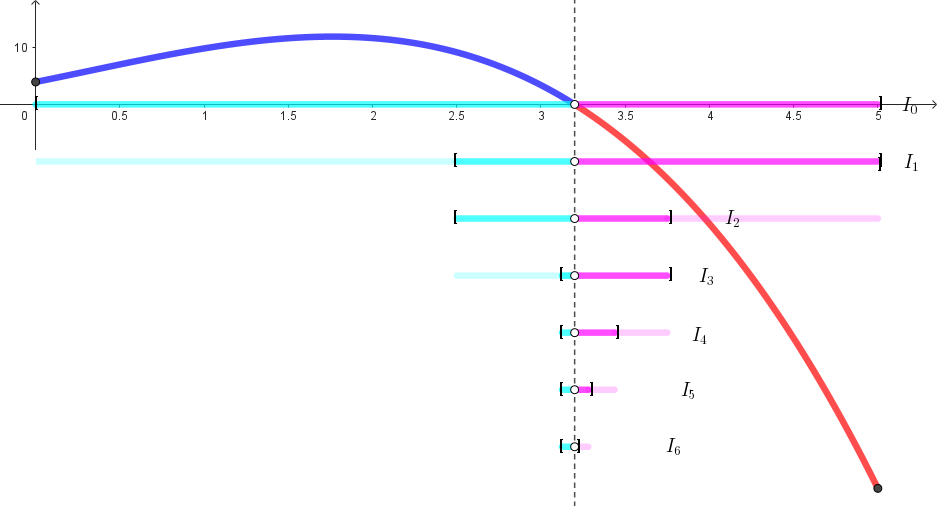
\includegraphics{IntervalosBolzano.png}

}

\caption{\label{fig-SeqInt}Sequência de Intervalos de Bolzano}

\end{figure}%

Para implementar esse algoritmo usaremos uma planilha eletrônica
seguindo os seguintes passos.

\begin{center}\rule{0.5\linewidth}{0.5pt}\end{center}

Dada uma função \(f(x)\) contínua em \([a,b]\) talque \(f(a)f(b)<0\).

\begin{enumerate}
\def\labelenumi{\arabic{enumi}.}
\tightlist
\item
  \textbf{Declaração das variáveis}:

  \begin{enumerate}
  \def\labelenumii{\alph{enumii})}
  \tightlist
  \item
    k (índice de iteração)
  \item
    ε (precisão de contas)
  \item
    PE (Ponta-Esquerda do Intervalo)
  \item
    PD (Ponta-Direita do Intervalo)
  \item
    x (Ponto de Corte)
  \item
    f(PE) (a imagem do PE)
  \item
    f(x) (a imagem do Ponto de Corte)
  \item
    Teste (Teste de Bolzano)
  \item
    ∆ (Passo)
  \end{enumerate}
\item
  \textbf{Entrada de valores/fórmulas}:

  \begin{enumerate}
  \def\labelenumii{\alph{enumii})}
  \tightlist
  \item
    k = 0 (índice 0 para valores iniciais)
  \item
    \(ε = 10^3\) (precisão adotada)
  \item
    PE = a
  \item
    PD = b
  \item
    x = (PE+PD)/2
  \item
    f(PE) (a imagem do PE)
  \item
    f(x) (a imagem do x)
  \item
    Teste = f(PE) f(x)
  \end{enumerate}
\item
  \textbf{Refinamento}

  \begin{enumerate}
  \def\labelenumii{\alph{enumii})}
  \tightlist
  \item
    NovoPE = Se(Teste\textless0, PE, x)
  \item
    NovoPD = Se(Teste\textless=0, x, PD)
  \item
    ∆ = \(abs(x_{1}-x_{0})\)
  \end{enumerate}
\end{enumerate}

\begin{center}\rule{0.5\linewidth}{0.5pt}\end{center}

Três observações a fazer. Primeiro, a razão de incluir 0 no Teste do
NovoPD é forçar que o novo intervalo seja {[}x,x{]}, tendo assim
comprimento zero quando o ponto de corte, x, é o próprio zero da função.
Com isso o processo terminaria. Segundo, para o Passo ∆ usamos o comando
\(abs(x_{1}-x_{0})\) que fornece o valor absoluto da diferença entre os
primeiros pontos médios. Por essa razão ele só pode ser definido a
partir da primeira iteração. Terceiro, na implementação em alguma
planilha eletrônica, não deve ser colocado os valores de cada variável,
mas os respectivos endereços na planilha.

Em planilha eletrônica o cabeçalho terá o seguinte aspecto

\begin{figure}[H]

{\centering 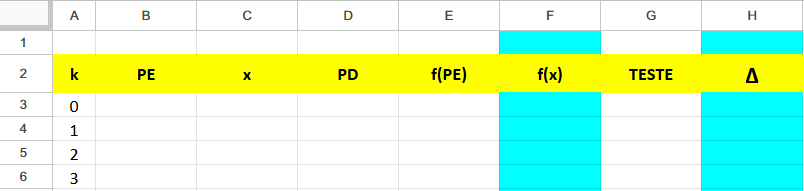
\includegraphics{CabBis.png}

}

\caption{Cabeçalho do Método da Bissecção}

\end{figure}%

As colunas F e H, em cor azulada, são os critérios de parada que
adotamos \[\begin{array}{ccc}
\left|f(x)\right|<\varepsilon & , & \Delta<\varepsilon\end{array}\] onde
\(\Delta=\left|x_{i+1}-x_{i}\right|\) medem os passos da melhora no
processo de aproximação ao zero da função. Quanto menor o passo, mais
perto estamos da raíz. Essas colunas azuladas devem ser monitoradas para
decidir se prosseguimos ou paramos com as iterações.Vamos entender
melhor apresentando um exemplo.

\textbf{Exemplo 1}. Método da Bissecção, ache o valor de \(\sqrt{15}\)
com precisão de 7 casas decimais corretas.

\textbf{Resolução}. Três passos iniciais precisam ser trilhados. O
primeiro é definir a função a zerar. Várias funções têm \$\sqrt{15}\$
como raíz, mas a mais simples delas talvez seja \[f(x)=x^{2}-15\] que é
a que vamos adotar. Em seguida, vamos definir o intervalo inicial de
Bolzano. Como
\[\underbrace{\sqrt{9}}_{3}<\sqrt{15}<\underbrace{\sqrt{16}}_{4}\] vamos
adotar \(I_{0}=[3,4]\). Por fim, como o enunciado pede 7 casas decimais
corretas, portanto \$\varepsilon=10\^{}\{-7\}\$, vamos trabalhar com 8
casas decimais, pensando que esta última casa decimal pode resultar de
um arredondamento, portanto imprecisa. A primeira linha ficaria assim

\begin{figure}[H]

{\centering 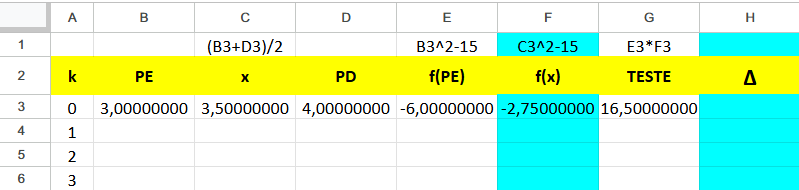
\includegraphics{CabBis1.png}

}

\caption{Primeira linha do Método da Bissecção}

\end{figure}%

Na segunda linha faremos a 1ª iteração e começaremos com o processo de
refinamento do Ponta Esquerda PE, na B4, e do Ponta Direita PD, na D4.

\begin{figure}[H]

{\centering 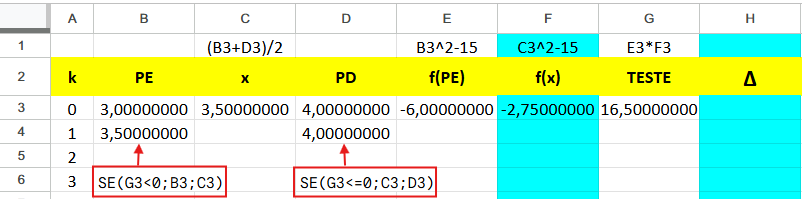
\includegraphics{CabBis2.png}

}

\caption{Refinamento do Método da Bissecção}

\end{figure}%

As células C4, E4, F4 e G4 serão cópias das C3, E3, F3 e G3,
respectivamente.

\begin{figure}[H]

{\centering 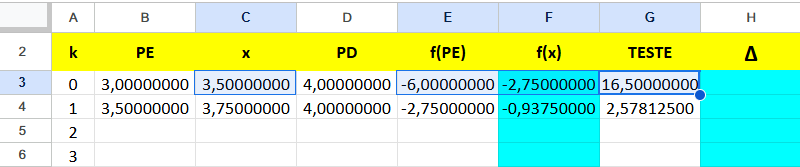
\includegraphics{CabBis2a.png}

}

\caption{Cópias da Linha anterior}

\end{figure}%

Finalmente completamos a linha 2 com o primeiro passo.

\begin{figure}[H]

{\centering 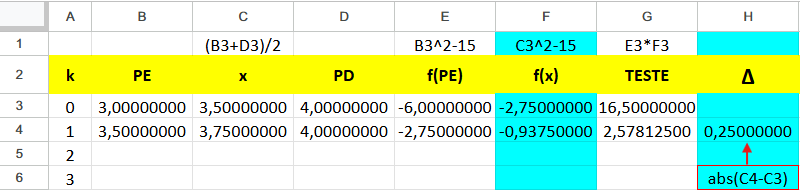
\includegraphics{CabBis2b.png}

}

\caption{Linha 2 do Método da Bissecção}

\end{figure}%

Feita a primeira iteração, as demais repetem o processo de refinamento.
Assim copiamos a linha 2 para as linhas abaixo e prestar atenção nas
colunas azuladas. Depois de 25 iterações obtemos o quadro da Figura
abaixo

\begin{figure}[H]

{\centering 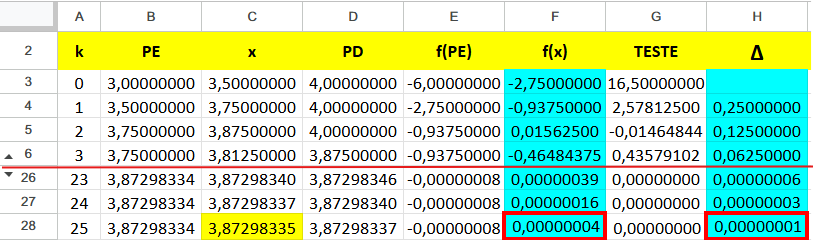
\includegraphics{CabBis3.png}

}

\caption{Método da Bissecção}

\end{figure}%

Observe que \[\begin{array}{c}
\mbox{F}28\,=\,0,00000004\,<0,0000001=\varepsilon\\
\mbox{H}28\,=\,0,00000001\,<0,0000001=\varepsilon
\end{array}.\]

Devemos assim monitorar as colunas azuladas para que os 7 primeiros
dígitos depois da vírgula sejam todos zeros. O resultado é o último
ponto médio, portanto \[x_{28}=\boldsymbol{3,8729833}\] lembrando que o
último dígito, 5, pode ser resultado de arredondamento, portanto não é
preciso.

\bookmarksetup{startatroot}

\chapter{Prefácio}\label{prefuxe1cio}

Este texto é escrito primeiramente para os alunos da disciplina de
Cálculo Numérico do Instituto Federal de Educação, Ciência e Tecnologia,
câmpus de Guarulhos. Mas é aberto a todos os interessados em conhecer
métodos numéricos usando uma didática diferenciada e usufruindo o que
temos hoje disponível no dia a dia: a tecnologia.

\bookmarksetup{startatroot}

\chapter{Summary}\label{summary}

In summary, this book has no content whatsoever.

\bookmarksetup{startatroot}

\chapter*{References}\label{references}
\addcontentsline{toc}{chapter}{References}

\markboth{References}{References}

\phantomsection\label{refs}
\begin{CSLReferences}{0}{1}
\end{CSLReferences}




\end{document}
